\section{Theorie}
\label{sec:Theorie}

Magnetische Felder werden von elektrischen Strömen und magnetischen Dipolen erzeugt.
Die Grundlage der Berechnung einer magnetischen Flussdichte $\symbf{B}$
am Ort $\symbf{r}$ durch einen stationären elektrischen Strom $I$ ist
das Biot-Savartsche Gesetz
\begin{equation}
  \symbf{B}(\symbf{r}) = \frac{\mu_0}{4 \symup{\pi}}
    \int_C \frac{I \symup{d} \symbf{s} \times \symbf{r}}{r^3}\,.
  \label{eqn:biotsavart}
\end{equation}
Dies ist ein Kurvenintegral über die stromdurchflossene Kurve $C$ mit ihrem
Wegelement $\symup{d}\symbf{s}$. Die magnetische Permeabilität des Vakuums $\mu_0$
hat den definierten Wert $\SI{4\pi e-7}{\henry\per\meter}$.

Eine Spule besteht aus einem gewickelten Draht, der auf einer Basis, meist einem Zylinder mit dem Radius $R$,
aufgebracht ist. Die Windungszahl $n$ drückt die Anzahl der Umläufe des Drahtes aus.
Eine von einem Strom $I$ durchflossene Spule erzeugt ein zur Stromstärke proportionales Magnetfeld.
Eine Skizze dazu ist in Abbildung \ref{fig:spule} zu sehen.

\begin{figure}
  \centering
  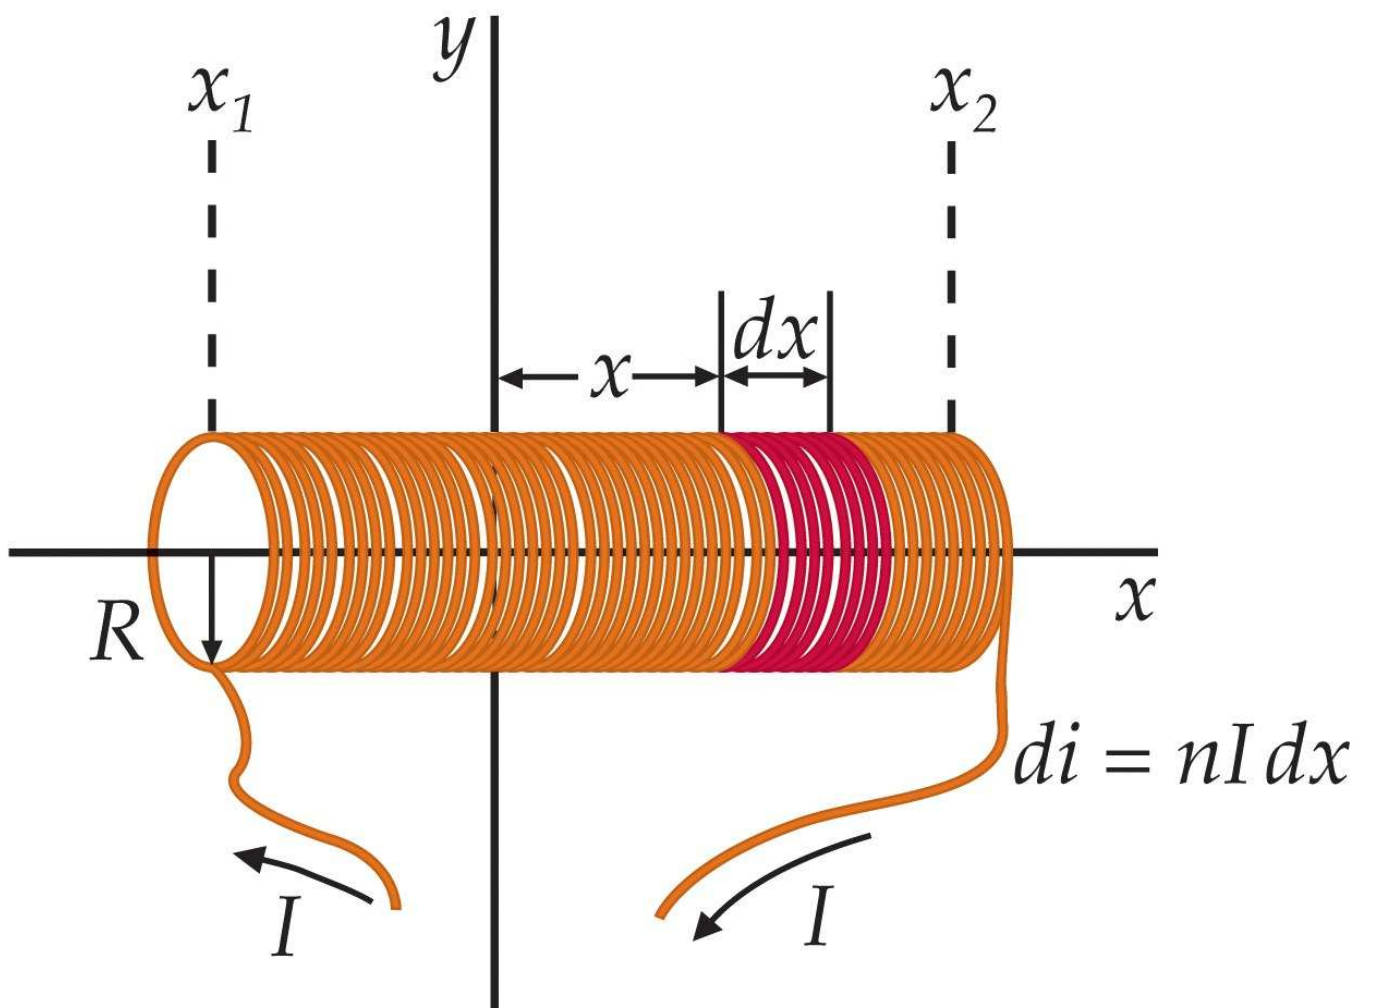
\includegraphics[width=300pt]{data/spule.png}
  \caption{Skizze einer Spule \cite{Spule}}
  \label{fig:spule}
\end{figure}

HIER NOCH DIE ABBILDUNG ERKLÄREN

Der Betrag der magnetischen Flussdichte so einer Spule auf ihrer Symmetrieachse lässt sich durch
\eqref{eqn:biotsavart} zu
\begin{equation}
  B_x(x) = \frac{\mu_0 n I}{2} \left( \frac{x-x_1}{\sqrt{(x-x_1)^2+R^2}} - \frac{x-x_2}{\sqrt{(x-x_2)^2+R^2}} \right)
\end{equation}
berechnen. Hierbei wurden abgesehen von einem verschwindenden Querschnitt keinerlei Näherungen vorgenommen.

Nähert man für eine Spule ihre Länge als deutlich größer gegenüber ihrem Durchmesser,
so ergibt sich näherungsweise für den Betrag der magnetischen Flussdichte durch Berechnung mit \eqref{eqn:biotsavart}
im Inneren der Spule
\begin{equation}
  B = \mu \frac{n}{l} I\,.
  \label{langespuleinnen}
\end{equation}
Dabei gilt für die Permeabilität $\mu = \mu_0 \mu_r$ mit der materialabhängigen
relativen Permeabilität $\mu_r$ und $l$ ist die Länge der Spule.
Die magnetische Flussdichte innerhalb der langen Spule ist ungefähr konstant, außerhalb
ist sie näherungsweise null.

Nahezu homogene Magnetfelder lassen sich mithilfe eines Helmholtz-Spulenpaars erzeugen.
Dieses besteht aus zwei in gleicher Richtung stromdurchflossenen Kreisspulen, die auf
auf einer gemeinsamen Achse aufgebaut werden. Ihr Abstand $d$ ist genau der gleiche Spulenradius $R$.
Auf der Symmetrieachse ist das Magnetfeld näherungsweise homogen. Sie lässt sich
ebenso mit dem Biot-Savartschen Gesetz \eqref{eqn:biotsavart} berechnen und ergibt sich zu


Die Messung magnetischer Felder geschieht in der Regel mithilfe einer Hall-Sonde.
In ihr befindet sich ein Metallplättchen, das von einem konstanten Strom durchflossen wird.
Ein äußeres magnetisches Feld übt Kraft auf die bewegten elektrischen Ladungen aus
und trennt sie. Dies erzeugt und eine Spannung und wird auch Hall-Effekt genannt.
Diese Spannung ist ein Maß für die Stärke der Flussdichte des äußeren magnetischen Feldes, welche
dann abgelesen werden kann. Je nach zu untersuchender Geometrie sind longitudinale und transversale Hall-Sonden
zu verwenden.
